\documentclass{beamer}
\title{EMQX Rebalancing and Node Evacuation}
\author{Ilya Averyanov}
\institute{EMQX}
\date{2022}
\usetheme{emqx}
\usepackage{listings}
\usepackage{color}
\usepackage{graphicx}
\usepackage{xcolor}
\usepackage{hyperref}
\definecolor{href}{rgb}{0,0,0.9375}
\hypersetup{
    pdfborderstyle={/S/U/W 1}, % underline links instead of boxes
    colorlinks=true,
    urlcolor=href
}
\lstset{frame=tb,
  aboveskip=3mm,
  belowskip=3mm,
  showstringspaces=false,
  columns=flexible,
  basicstyle={\small\ttfamily},
  numbers=none,
  numberstyle=\tiny\color{gray},
  keywordstyle=\color{blue},
  commentstyle=\color{dkgreen},
  stringstyle=\color{mauve},
  breaklines=true,
  breakatwhitespace=false,
  tabsize=2
}


\begin{document}

\frame{\titlepage}

% \begin{frame}
%     \frametitle{feature}
%     \framesubtitle{Externally}

%     \begin{itemize}
%         \item Each topic can have a \textit{retained} message
%         \item This message is sent to each subscriber on topic subscribe
%         \item A subscriber can subscribe to many topics at once using wildcards and receive many
%         retained messages
%     \end{itemize}

%     \begin{center}
%         \includegraphics[width=10cm, keepaspectratio]{images/retain-demo.png}
%     \end{center}
%     \lstinline{DeviceModel} and \lstinline{Owner}.

%     \vspace{1cm}

%     \begin{lstlisting}
%       lst
%     \end{lstlisting}

% \end{frame}

\begin{frame}
    \frametitle{Node Evacuation}
    \framesubtitle{Problem}

    \begin{center}
        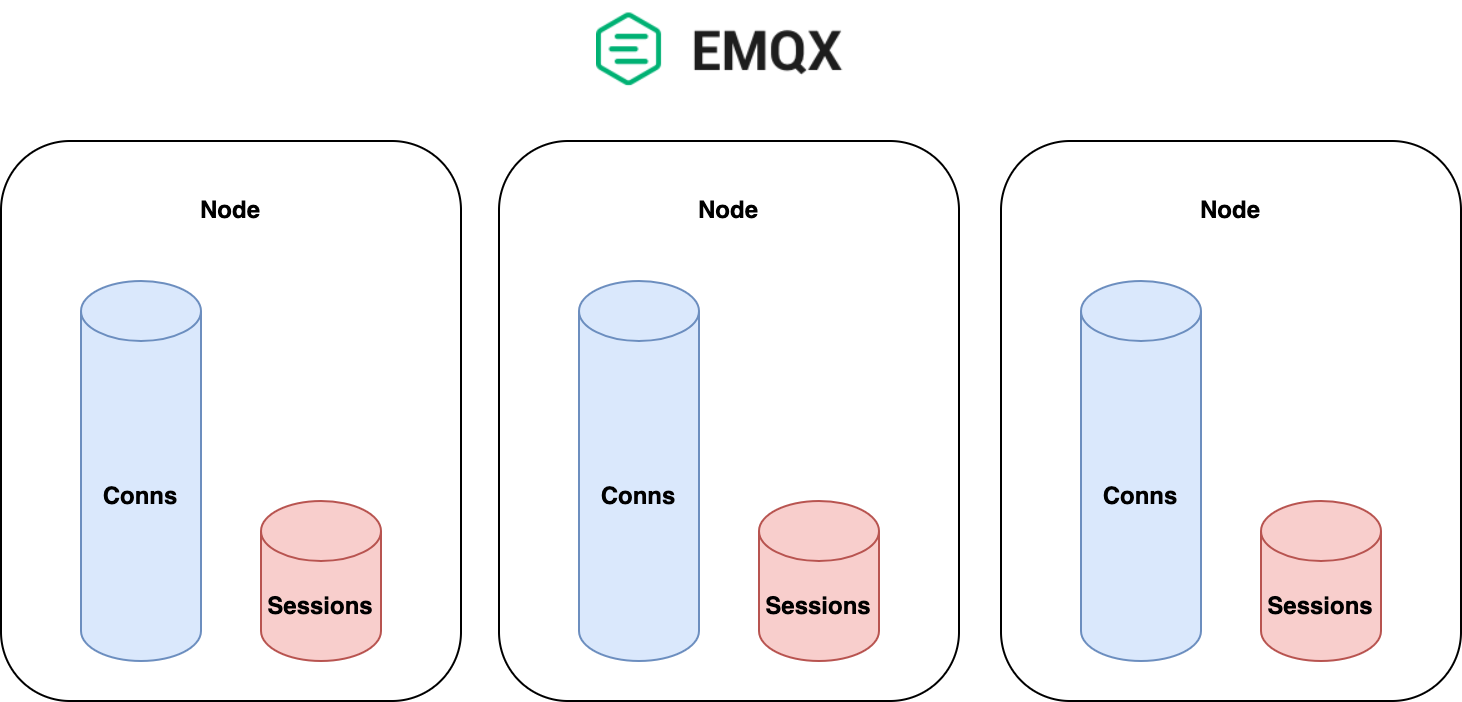
\includegraphics[width=8cm, keepaspectratio]{images/evacuation-scheme0.png}
    \end{center}
\end{frame}

\begin{frame}
    \frametitle{Node Evacuation}
    \framesubtitle{Problem}

    \begin{center}
        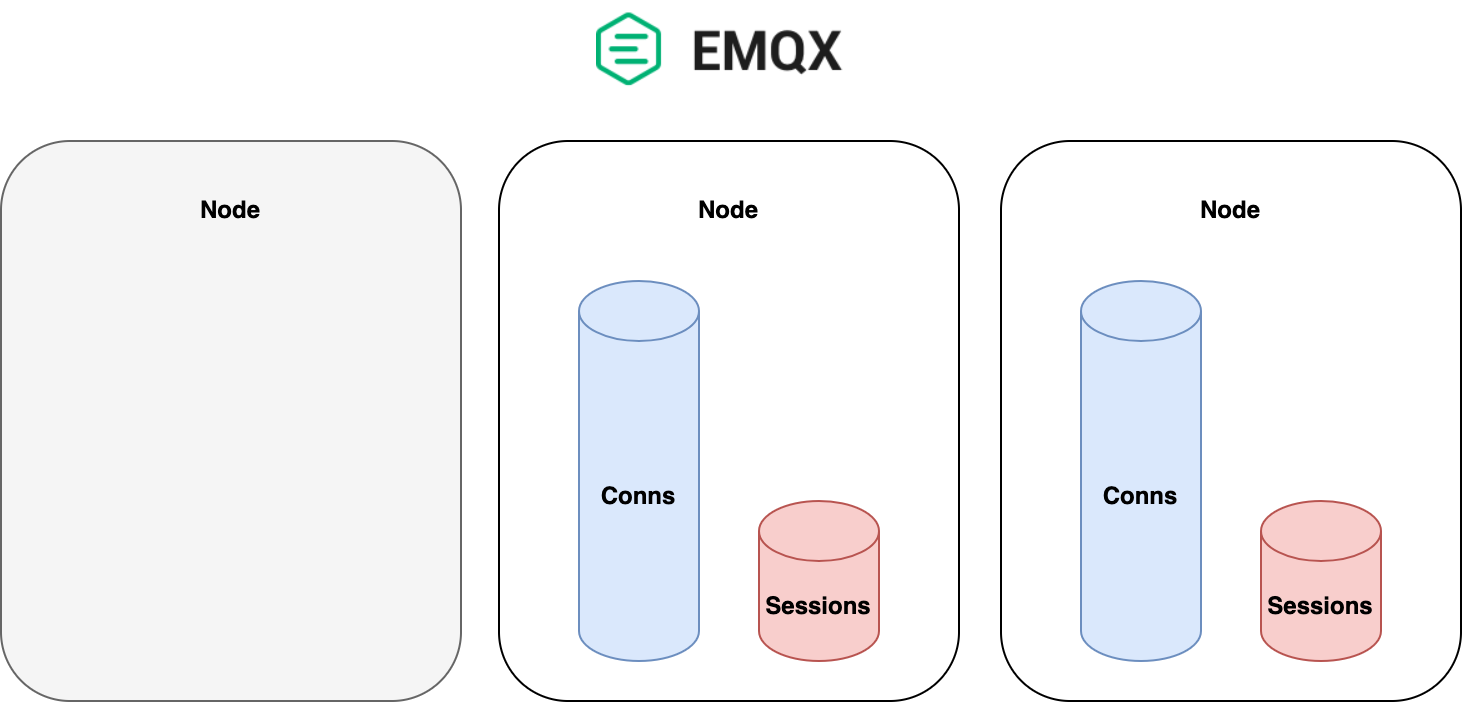
\includegraphics[width=8cm, keepaspectratio]{images/evacuation-scheme1.png}
    \end{center}
\end{frame}

\begin{frame}
    \frametitle{Node Rebalance}
    \framesubtitle{Problem}

    \begin{center}
        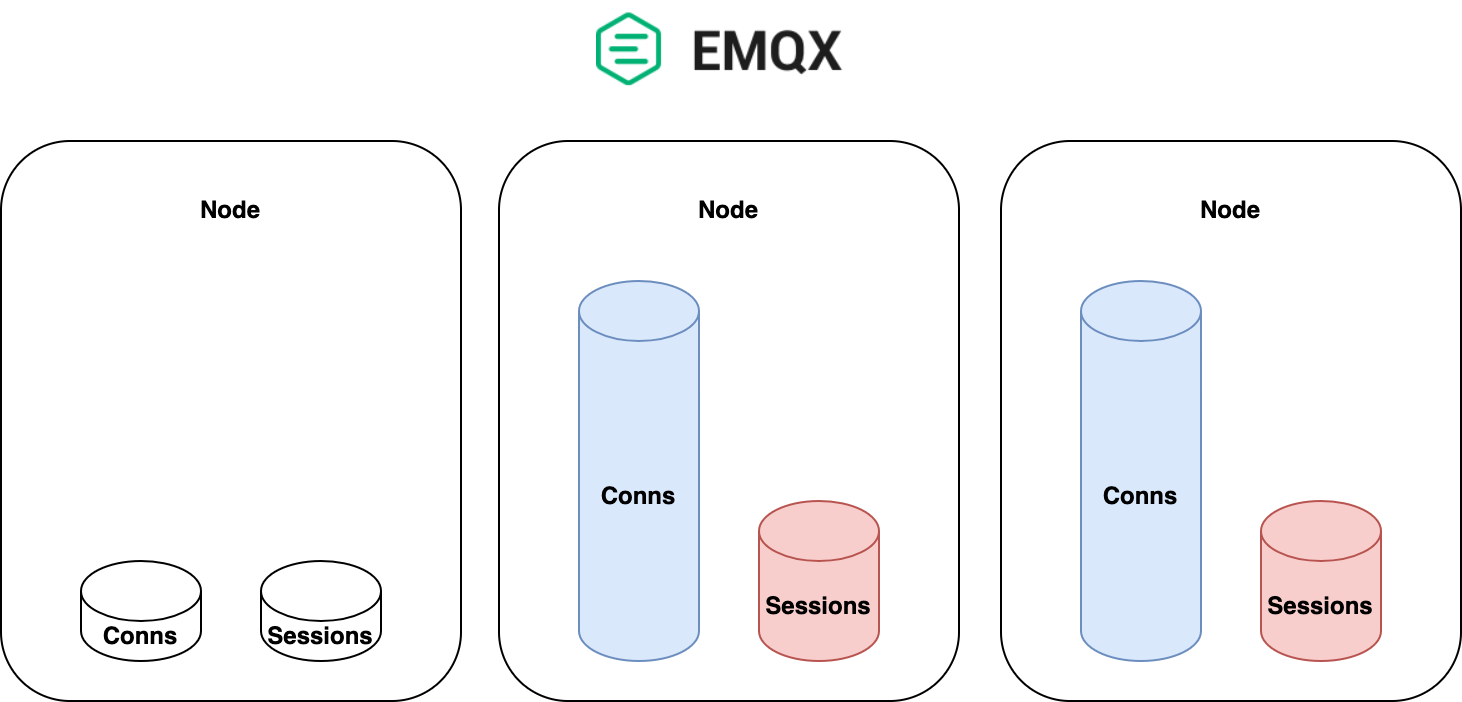
\includegraphics[width=8cm, keepaspectratio]{images/rebalance-scheme.png}
    \end{center}
\end{frame}

\begin{frame}
    \frametitle{Node Rebalance}
    \framesubtitle{Solution}

    We introduce two new apps:
    \begin{itemize}
        \item \lstinline{emqx_eviction_agent} -- low-level logic
        \item \lstinline{emqx_node_rebalance} -- high-level scenarios
    \end{itemize}
\end{frame}

\begin{frame}
    \frametitle{EMQX Eviction Agent}
    \begin{center}
        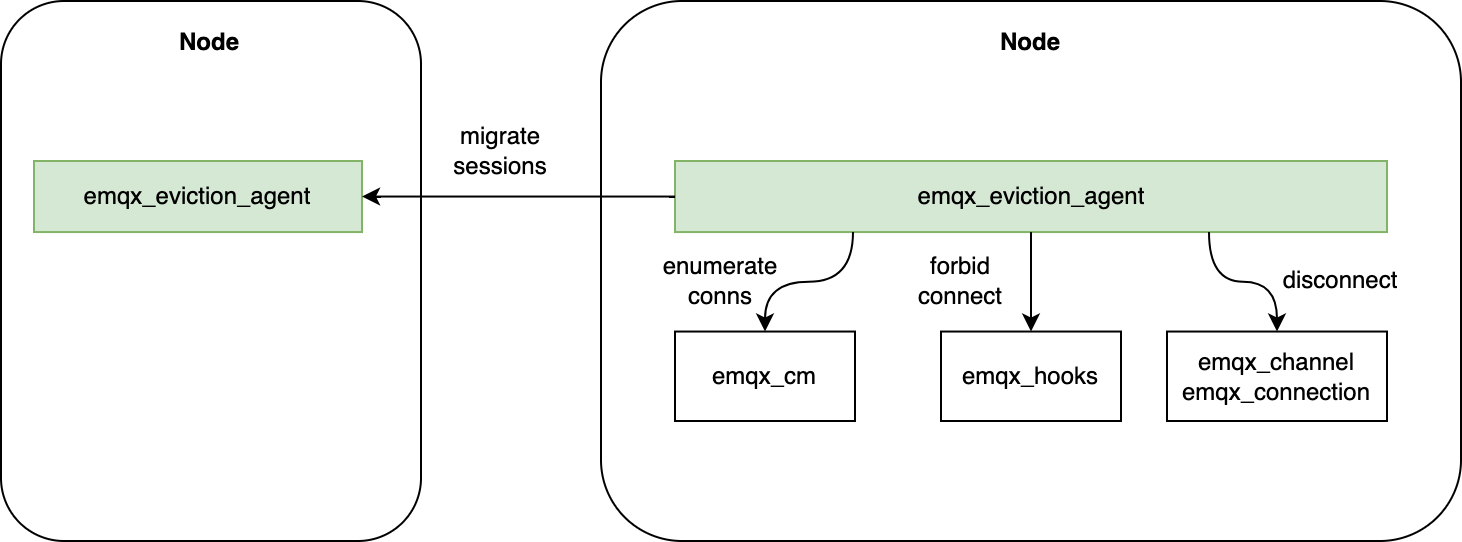
\includegraphics[width=8cm, keepaspectratio]{images/eviction-agent.png}
    \end{center}
\end{frame}

\begin{frame}
    \frametitle{EMQX Node Rebalance}
    \begin{center}
        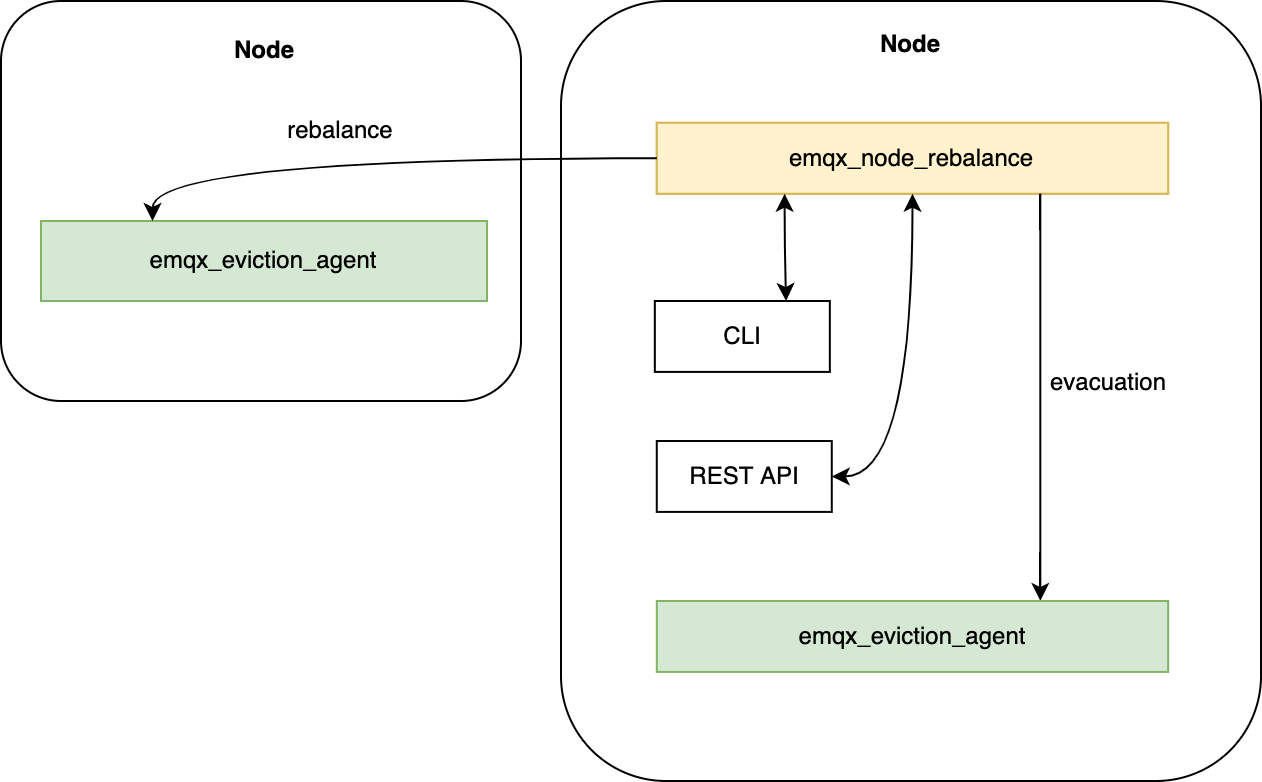
\includegraphics[width=8cm, keepaspectratio]{images/node-rebalance.png}
    \end{center}
\end{frame}

\begin{frame}
    \frametitle{EMQX Node Rebalance}
    \framesubtitle{Scenarios}
    \begin{itemize}
        \item Node evacuation
        \item Node rebalance
    \end{itemize}
\end{frame}

\begin{frame}
    \frametitle{EMQX Node Evacuation}
    \framesubtitle{Algorithm}
    \begin{center}
        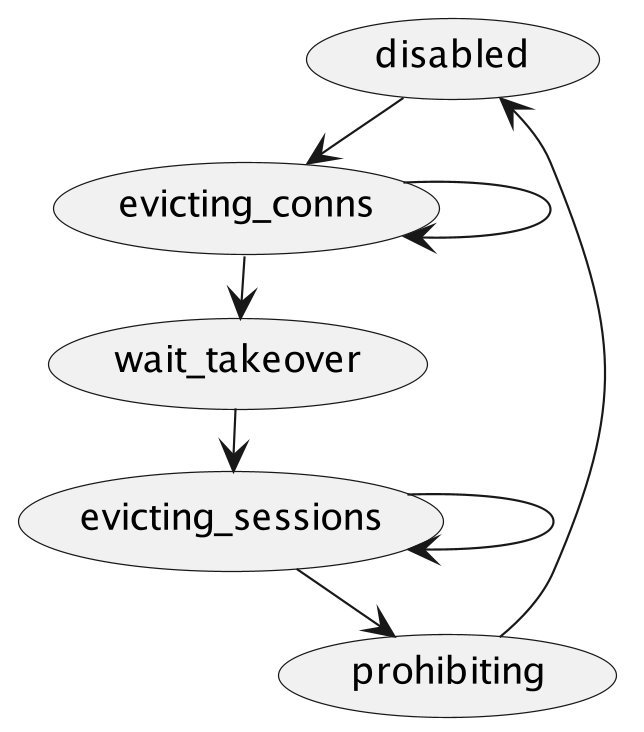
\includegraphics[height=6cm, keepaspectratio]{images/evacuation.png}
    \end{center}
\end{frame}

\begin{frame}
    \frametitle{EMQX Node Rebalance}
    \framesubtitle{Algorithm}
    \begin{center}
        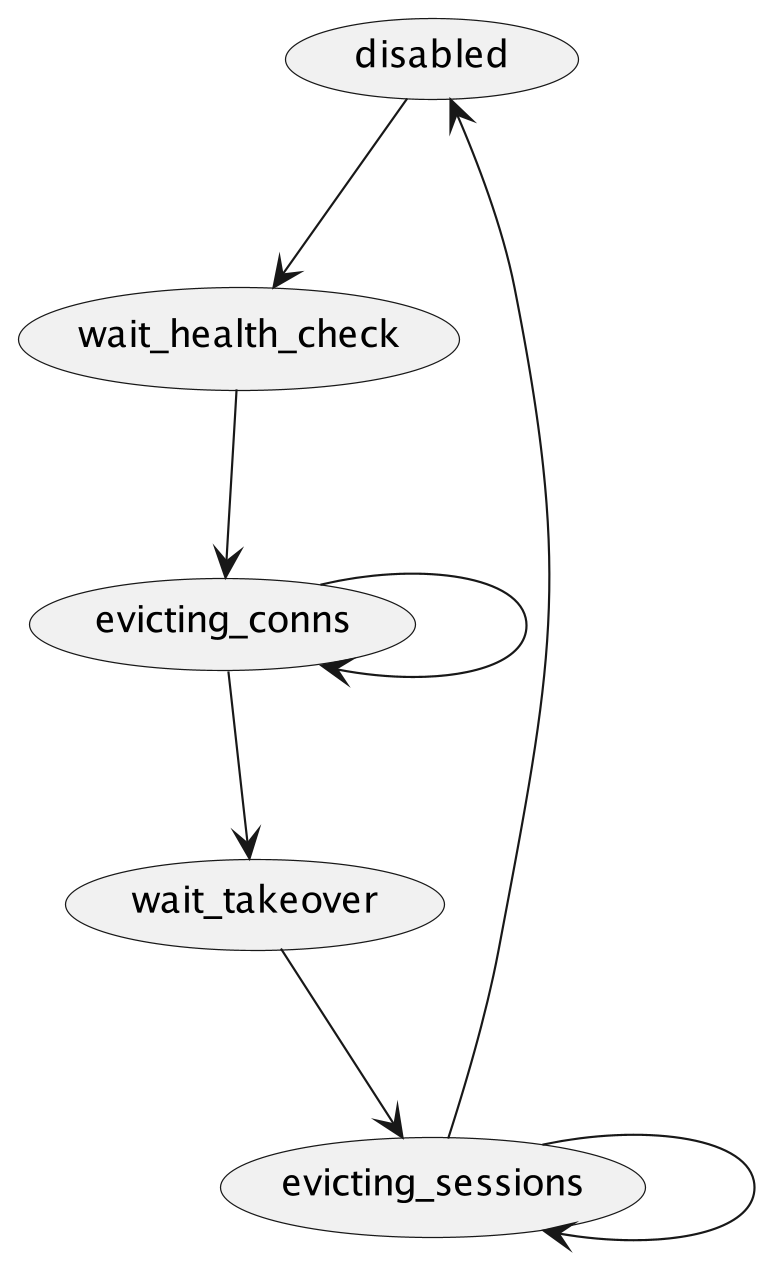
\includegraphics[height=6cm, keepaspectratio]{images/rebalance.png}
    \end{center}
\end{frame}

\begin{frame}
    \frametitle{EMQX Node Rebalance}
    \framesubtitle{Algorithm}
    \begin{center}
        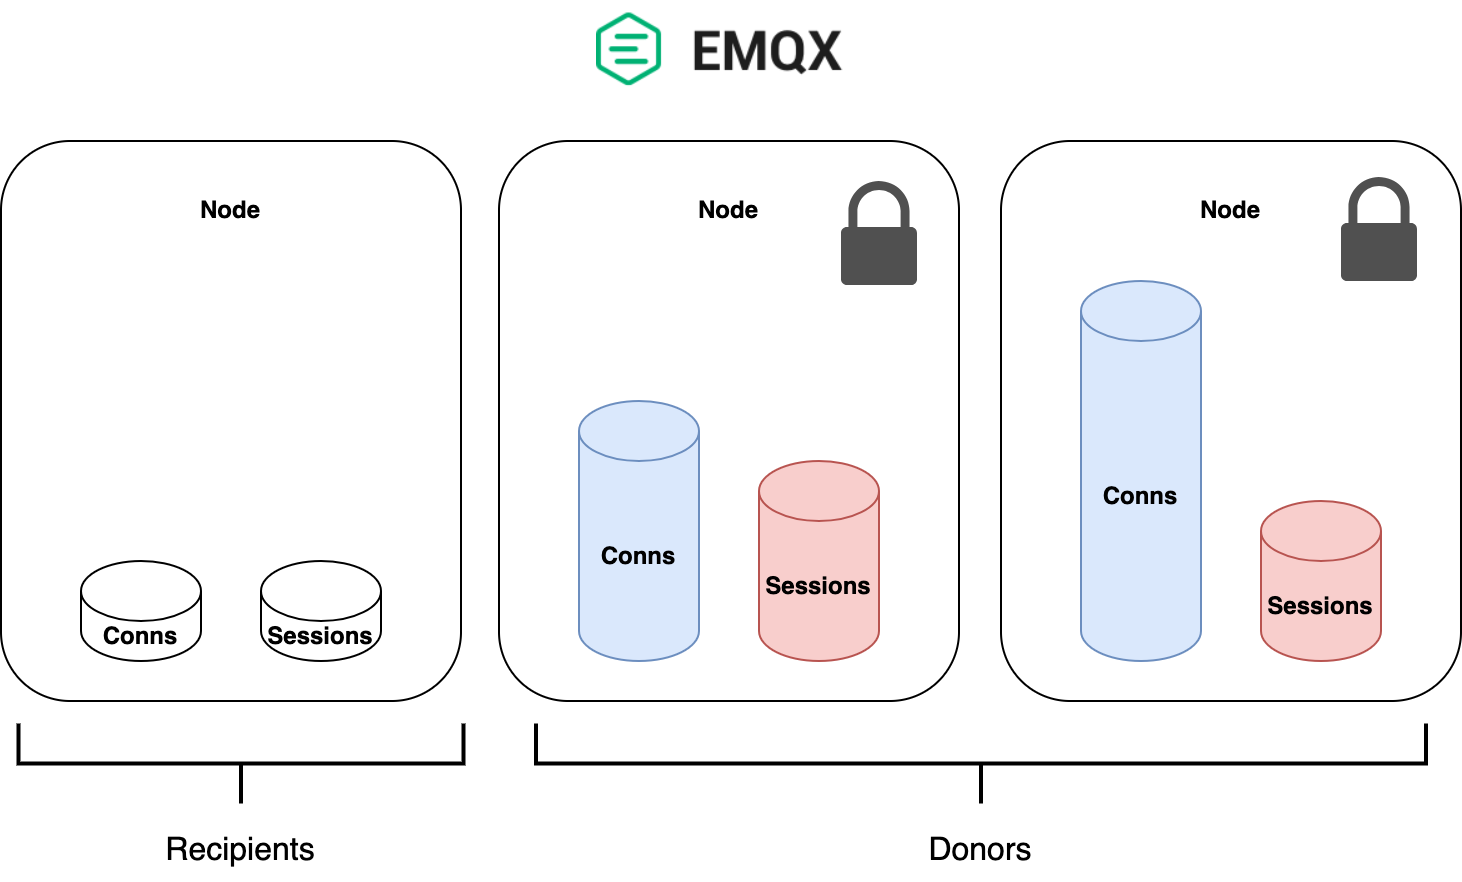
\includegraphics[width=8cm, keepaspectratio]{images/node-rebalance-algo0.png}
    \end{center}
\end{frame}

\begin{frame}
    \frametitle{EMQX Node Rebalance}
    \framesubtitle{Algorithm}
    \begin{center}
        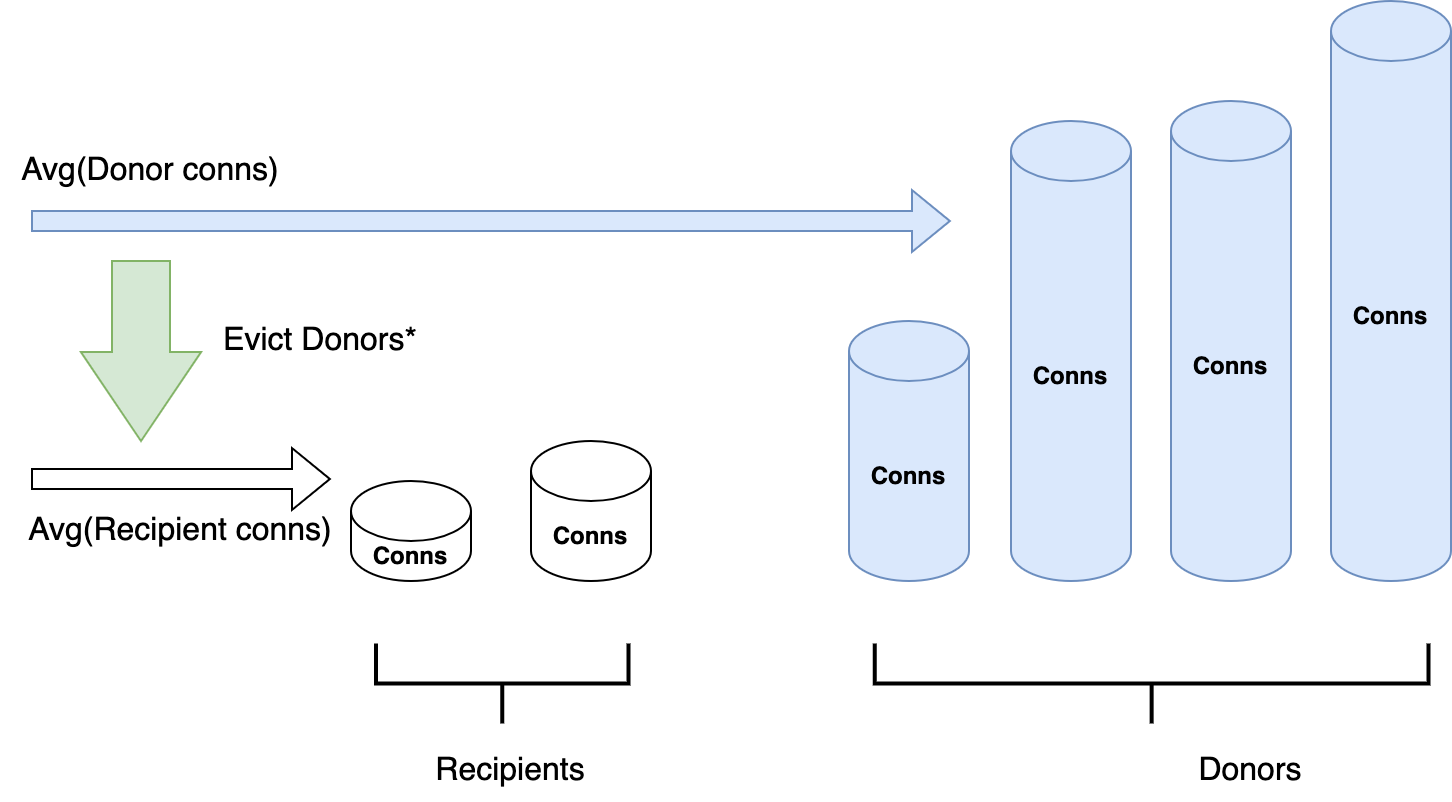
\includegraphics[width=8cm, keepaspectratio]{images/node-rebalance-algo1.png}
    \end{center}
\end{frame}

\begin{frame}
    \frametitle{EMQX Node Rebalance}
    \framesubtitle{Scenarios}
    \begin{itemize}
        \item We suppose that connection are distributed among new nodes evenly
        \item We do not evict from donors that have too few connections/sessions
    \end{itemize}
\end{frame}

\begin{frame}
    \frametitle{EMQX Node Rebalance}
    \framesubtitle{Algorithm}
    \begin{center}
        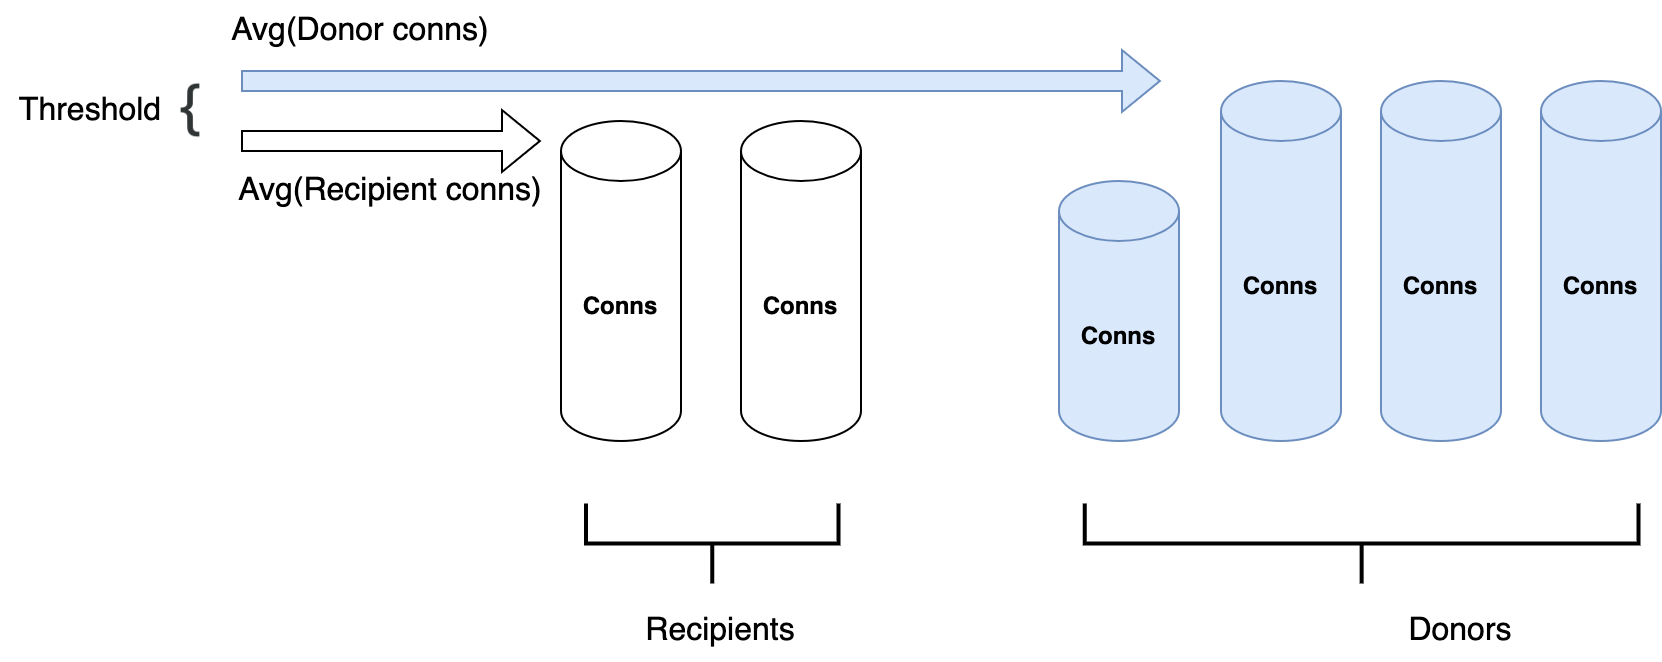
\includegraphics[width=8cm, keepaspectratio]{images/node-rebalance-algo2.png}
    \end{center}
\end{frame}

\begin{frame}
    \begin{center}
        Thank you!
    \end{center}
\end{frame}

\end{document}
